% 编译方式：XeLaTeX；图片均相对于本文件所在目录引用。
\documentclass[12pt,a4paper,fontset=fandol]{ctexart}
\usepackage[margin=2.2cm]{geometry}
\usepackage{graphicx}
\usepackage{booktabs}
\usepackage{amsmath}
\usepackage{float}
\usepackage{hyperref}
\usepackage{xcolor}
\usepackage{listings}
\usepackage{array}
\usepackage{caption}

\hypersetup{hidelinks}
\captionsetup{font=small}
\graphicspath{{images/}}
\setlength{\emergencystretch}{2em}
\renewcommand{\arraystretch}{1.18}
\lstset{
  language=Verilog,
  basicstyle=\ttfamily\footnotesize,
  keywordstyle=\color{blue!70!black},
  commentstyle=\color{green!40!black},
  stringstyle=\color{orange!60!black},
  showstringspaces=false,
  breaklines=true,
  breakatwhitespace=false,
  columns=fullflexible,
  keepspaces=true,
  frame=single,
  numbers=left,
  numberstyle=\tiny\color{gray},
  numbersep=7pt,
  xleftmargin=1.5em,
  framexleftmargin=0.4em,
  tabsize=4,
  captionpos=t
}

% 保留模板中的个人信息填写栏，不代填未知信息。
\newcommand{\reporttitle}{实验一：组合电路设计}
\newcommand{\subtask}{基础门电路、复用器、编码器与译码器}
\newcommand{\authname}{姓名}
\newcommand{\authid}{学号}
\newcommand{\class}{班级}

\title{\reporttitle\\[0.5em]\large\subtask}
\author{\authname：\underline{李祥熙}\quad
        \authid：\underline{2234412799}\quad
        \class：\underline{计算机2301}}
\date{2026年10月23日}

\begin{document}
\maketitle
\tableofcontents
\newpage

\section{实验目的}

本实验围绕组合逻辑电路展开，学习从逻辑表达式、真值表和硬件描述语言三个角度描述同一功能。具体目标如下：
\begin{itemize}
  \item 掌握与、或、非、与非等基本逻辑门的连接方法，并用完整真值表检查多输入表达式。
  \item 理解二选一和四选一复用器的选择关系，通过复用子电路掌握层次化设计方法。
  \item 理解普通编码器与优先编码器的区别，明确优先级、使能和有效状态信号的作用。
  \item 使用 Verilog 实现二线四线译码器、三线八线译码器和八线三线优先编码器，掌握连续赋值和组合逻辑过程块。
  \item 编写自动检查结果的测试平台，结合仿真波形、控制台输出和穷举测试判断设计是否符合预期。
\end{itemize}

\section{实验过程}

\subsection{实验环境}

\begin{itemize}
  \item 操作系统：Windows。
  \item 图形化电路工具：Logisim-evolution 3.8.0。
  \item 硬件描述语言与仿真工具：Verilog、Vivado 2026.1 及其自带的 XSim。
  \item Vivado 工程目标器件：\texttt{xc7a35tcsg324-1}，属于 Artix-7 系列。
  \item 验证方式：Logisim 组合分析与 Vivado RTL 行为仿真。
\end{itemize}

本实验中的电路都不包含时钟、触发器或存储单元。输出由当前输入决定，测试平台中的时间间隔用于安排测试激励。现有实验记录验证的是逻辑功能，没有给出 FPGA 下载、资源占用或布局布线后时序测试结果。

\subsection{实验任务与测试输入}

讲义介绍了多输入门电路、复用器、编码器和译码器，并允许使用 Vivado 或 Logisim 完成设计与验证。本次采用两种工具结合的方式：先在 Logisim 中完成门电路和复用器，再在 Vivado 中练习译码器和优先编码器的 Verilog 设计。

\begin{table}[H]
\centering
\caption{本次实验的实现内容与验证范围}
\label{tab:scope}
\small
\begin{tabular}{p{3.0cm}p{3.5cm}p{8.0cm}}
\toprule
电路 & 实现方式 & 验证范围 \\
\midrule
多输入门电路 & Logisim 基本逻辑门 & 五个一位输入，共 32 种组合 \\
二选一复用器 & Logisim 基本逻辑门 & 两个数据输入和一个选择输入，共 8 种组合 \\
四选一复用器 & 三个二选一子电路 & 四个数据输入和两个选择输入，共 64 种组合 \\
优先编码器组件 & Logisim 内置组件 & 八位输入及使能，共 512 种组合的折叠真值表 \\
二线四线译码器 & Verilog 连续赋值 & 全部 4 种二进制输入，40 ns \\
三线八线译码器 & Verilog 连续赋值 & 全部 8 种二进制输入，80 ns \\
八线三线优先编码器 & Verilog 组合过程块 & 全部 256 种二进制输入，2560 ns \\
\bottomrule
\end{tabular}
\end{table}

表\ref{tab:scope}中的组合数由输入位数确定。例如，四选一复用器共有六个一位输入，因此完整真值表有 $2^6=64$ 行。Logisim 截图中的折叠显示会合并输出相同且部分输入无关的行，显示行数减少不表示输入空间缩小。Verilog 的三组测试均对相应输入空间进行穷举，但只覆盖确定的二进制输入，不包含未知态或高阻态输入的专项测试。

普通八线三线编码器用于理解编码原理，本次没有单独保存它的实现与测试结果；三态缓冲器复用器属于讲义中的选做内容，本次未实现。译码功能采用 Verilog 验证，现有材料没有另外记录 Logisim 内置译码器的使能测试。

\subsection{实现步骤}

\begin{enumerate}
  \item 阅读讲义，明确每个电路的输入、输出、逻辑表达式和有效条件。
  \item 在 Logisim 中建立多输入门电路和二选一复用器，设置引脚方向与位宽，通过组合分析生成真值表。
  \item 将二选一复用器作为子电路，在四选一电路中放置三个实例，连接两级选择网络并检查真值表。
  \item 放置 Logisim 优先编码器，通过八位总线和分线器连接数据输入，补充使能及状态输出引脚。
  \item 在 Vivado 中建立 RTL 工程，将三个电路加入设计源，将对应测试平台加入仿真源。每次仿真前将相应测试平台设为仿真顶层。
  \item 为译码器生成单热期望值，为优先编码器计算最高有效位编号；每组输入保持 10 ns，再比较实际输出与期望值。
  \item 检查输出波形和结束提示。优先编码器运行超过默认的 1000 ns 时，使用 \texttt{run all} 继续至测试结束。
\end{enumerate}

上述流程把功能设计和测试检查分开。设计源描述待实现的硬件；测试平台中的循环、延时和输出语句用于仿真控制，不作为待下载的电路。报告编写时还在独立临时目录中使用本机 XSim 对现有六份源文件重新编译并运行三个测试平台，用于复核截图中的结论。

\section{实验内容}

\subsection{任务一：多输入门电路}

讲义要求实现的函数为
\begin{equation}
  x=\overline{a\cdot\overline b\cdot c\cdot(d+e)}.
\end{equation}
其中乘号表示逻辑与，加号表示逻辑或，横线表示逻辑非。只有括号内所有与条件都成立时，输出才为零。

实际电路将最后两个输入标为 $e$ 和 $f$。为与截图及保存的电路一致，本文使用实际引脚名称：
\begin{equation}
  x=\overline{a\cdot\overline b\cdot c\cdot(e+f)}.
  \label{eq:gate}
\end{equation}
式\eqref{eq:gate}中的实际输入 $e$ 对应讲义中的 $d$，实际输入 $f$ 对应讲义中的 $e$，只是重命名，逻辑结构不变。

实现时，先对 $b$ 取反，将 $a,\overline b,c$ 接入三输入与门；将 $e,f$ 接入或门；最后用与非门连接这两条支路。使用与非门可以直接完成最后一级与运算和输出取反。

输出为零的必要且充分条件为
\begin{equation}
  a=1,\quad b=0,\quad c=1,\quad (e,f)\in\{(0,1),(1,0),(1,1)\}.
\end{equation}
因此 32 组输入中应有 3 组输出为零，其余 29 组输出为一。这个数量关系可以用来快速检查完整真值表，而不仅观察某一个输入状态。

\subsection{任务二：二选一复用器}

二选一复用器包括数据输入 $D_0,D_1$、选择输入 $S$ 和输出 $Y$，其表达式为
\begin{equation}
  Y=D_0\overline S+D_1S.
\end{equation}
当 $S=0$ 时，第一条支路传递 $D_0$；当 $S=1$ 时，第二条支路传递 $D_1$。两条支路通过或门合并输出。

电路由一个非门、两个与门和一个或门组成。所有引脚均为一位，不需要时钟和使能输入。验证时遍历 $D_0,S,D_1$ 的八种组合，确认未被选择的数据输入不会影响输出。

\subsection{任务三：利用子电路实现四选一复用器}

四选一复用器采用两级结构。第一级使用两个二选一实例，第二级再用一个二选一实例：
\begin{align}
  A &= D_0\overline{S_0}+D_1S_0,\\
  B &= D_2\overline{S_0}+D_3S_0,\\
  Y &= A\overline{S_1}+BS_1.
\end{align}
其中 $S_0$ 在每一组数据内选择，$S_1$ 决定选择上组还是下组。展开后得到
\begin{equation}
  Y=D_0\overline{S_1}\overline{S_0}
    +D_1\overline{S_1}S_0
    +D_2S_1\overline{S_0}
    +D_3S_1S_0.
\end{equation}
这说明 $S_1$ 为高位选择信号，$S_0$ 为低位选择信号；两位选择码对应四个数据输入的编号。

\begin{table}[H]
\centering
\caption{四选一复用器的选择关系}
\label{tab:mux4}
\begin{tabular}{ccc}
\toprule
$S_1$ & $S_0$ & 输出 $Y$ \\
\midrule
0 & 0 & $D_0$ \\
0 & 1 & $D_1$ \\
1 & 0 & $D_2$ \\
1 & 1 & $D_3$ \\
\bottomrule
\end{tabular}
\end{table}

表\ref{tab:mux4}表示每个选择码下只有一个数据输入有效，其余三个数据输入可以任意改变。在 Logisim 中先打开四选一电路，再单击左侧已有的二选一电路即可放置子电路实例。该方法复用了已经验证的基本模块，也使选择信号的分工更清晰。

\subsection{任务四：普通编码与优先编码原理}

普通八线三线编码器假定八个输入中恰有一个为一，输出为该输入的编号。例如，只有 $I_5=1$ 时输出为二进制 $101$。在这个单热输入条件下，有
\begin{align}
  Y_2&=I_4+I_5+I_6+I_7,\\
  Y_1&=I_2+I_3+I_6+I_7,\\
  Y_0&=I_1+I_3+I_5+I_7.
\end{align}
这些表达式仅在满足输入约束时具有编码意义。例如 $I_1$ 和 $I_2$ 同时为一时，直接使用上述或表达式会得到 $011$，无法解释为两者中某个输入的编号。优先编码器通过规定优先顺序解决这个问题。

本实验采用 $I_7$ 最高、$I_0$ 最低的优先顺序。当输入非零时，其功能可表示为
\begin{equation}
  Y=\max\{j\mid I_j=1,\ 0\leq j\leq7\}.
\end{equation}
该式输出最高有效位的编号，而不是输入中一的数量。输入为零时没有有效编号，需要另外规定默认输出或提供有效状态信号。

\subsubsection{Logisim 内置优先编码器}

Logisim 中设置三位选择宽度，得到八个数据输入和三位编码输出。通过八位输入引脚与分线器，将总线位 $I[0]$ 至 $I[7]$ 分别连接到对应编号的输入端，同时连接使能和状态引脚。

\begin{table}[H]
\centering
\caption{Logisim 优先编码器各信号的含义}
\label{tab:priority-ports}
\begin{tabular}{cp{12.0cm}}
\toprule
信号 & 含义 \\
\midrule
$I[7:0]$ & 八位数据输入，高位优先 \\
$EN$ & 高电平使能 \\
$Y[2:0]$ & 最高有效输入的三位编号 \\
$C$ & 组有效信号，使能且存在有效输入时为一 \\
$F$ & 级联使能输出，使能且全部数据输入为零时为一 \\
\bottomrule
\end{tabular}
\end{table}

表\ref{tab:priority-ports}中，$C$ 可用于判断编码结果是否有效，$F$ 可用于级联。对于确定的二进制输入，可以写为 $C=EN\cdot(I_0+\cdots+I_7)$、$F=EN\cdot\overline{(I_0+\cdots+I_7)}$。当 $EN=1$ 且所有输入为零时，真值表将 $Y$ 标为无关项；当 $EN=0$ 时，截图中的组件输出 $F=0,C=0,Y=000$。

\subsubsection{Verilog 优先编码器}

Verilog 模块只保留八位输入 \texttt{i} 和三位输出 \texttt{y}，使用从高位到低位的 \texttt{if/else if} 链进行判断。最高位满足后就不再执行后续分支，从而形成优先关系。完整源码见附录，关键结构如下：

\begin{lstlisting}[caption={优先编码器的组合逻辑结构}]
always @* begin
    if      (i[7]) y = 3'd7;
    else if (i[6]) y = 3'd6;
    else if (i[5]) y = 3'd5;
    else if (i[4]) y = 3'd4;
    else if (i[3]) y = 3'd3;
    else if (i[2]) y = 3'd2;
    else if (i[1]) y = 3'd1;
    else          y = 3'd0;
end
\end{lstlisting}

上述代码用 \texttt{always @*} 自动包含相关输入的变化，并在组合过程块中使用阻塞赋值。每条执行路径都会给 \texttt{y} 赋值，因此不需要保持旧值，不会因分支遗漏而推断出锁存器。\texttt{output reg} 说明它接受过程赋值，并不表示电路中一定存在寄存器。

最后的默认分支同时覆盖只有 $i[0]=1$ 和全部输入为零两种情况，因此这两种输入均输出零。该模块没有 $EN,C,F$ 端口，与 Logisim 组件比较时，只能对使能且至少存在一个有效输入的编码结果直接比较；全零输入则遵循本模块明确给出的默认值。

\subsection{任务五：二线四线译码器}

译码器将二进制编号转换成单热输出。二线四线译码器的输入为 \texttt{a[1:0]}，输出为 \texttt{y[3:0]}，高电平表示选中：
\begin{align}
  y_0&=\overline{a_1}\,\overline{a_0},&
  y_1&=\overline{a_1}a_0,\\
  y_2&=a_1\overline{a_0},&
  y_3&=a_1a_0.
\end{align}
每个输出是输入变量的一个最小项；对于确定的二进制输入，只有一个最小项成立。源码分别用四条 \texttt{assign} 描述这四个条件，所有输出均为 \texttt{wire}，也没有额外的使能条件。

测试平台遍历输入 $0,1,2,3$，使用移位运算生成期望值：
\begin{lstlisting}[caption={二线四线译码器的期望值生成和检查}]
a = k;
expected = 4'b0001 << k;
#10;
if (y !== expected) begin
    $display("FAIL: a=%b y=%b expected=%b",
             a, y, expected);
    $fatal(1, "decoder2 failed");
end
\end{lstlisting}

这里用移位方法生成单热期望值，与设计中的逐位逻辑表达式采用不同形式，便于交叉检查。等待 10 ns 后再比较，可以让待测组合逻辑在仿真调度中完成更新。\texttt{!==} 是四态比较中的不全等运算，若实际输出出现未知值或高阻值，也会相对于确定的期望值判定为不匹配。

\subsection{任务六：三线八线译码器}

三线八线译码器输入为 \texttt{a[2:0]}，输出为 \texttt{y[7:0]}。对每个 $j\in\{0,\ldots,7\}$，当输入数值等于 $j$ 时，仅 $y_j=1$；其他输出为零。例如：
\begin{equation}
  y_0=\overline{a_2}\overline{a_1}\overline{a_0},\qquad
  y_5=a_2\overline{a_1}a_0,\qquad
  y_7=a_2a_1a_0.
\end{equation}
这三个输出分别对应二进制编号 $000,101,111$。完整实现对八个最小项逐条连续赋值，保证三位输入的全部组合均有定义。

测试平台遍历 $0$ 至 $7$，使用 \texttt{8'b00000001 << k} 产生期望输出，每组等待 10 ns 后比较。与二线四线译码器相比，测试结构保持不变，只扩展了输入位宽、输出位宽和枚举范围；总仿真时间为 $8\times10=80$ ns。

\subsection{测试平台与仿真时间的安排}

三组测试平台都使用 1 ns 时间单位和 1 ps 时间精度。测试信号由过程块驱动，因此声明为 \texttt{reg}；待测模块输出连接到 \texttt{wire}。\texttt{dut} 是被测模块的实例名，\texttt{.a(test\_input)} 等命名端口连接可以避免位置连接造成的顺序错误。

优先编码器的期望值采用从低位向高位扫描的方法：
\begin{lstlisting}[caption={现有优先编码器测试平台中的期望值计算}]
expected = 3'b000;
for (k = 0; k < 256; k = k + 1) begin
    test_input = k;
    for (bit_index = 0; bit_index < 8;
         bit_index = bit_index + 1) begin
        if (test_input[bit_index]) expected = bit_index;
    end
    #10;
    // Compare test_output with expected here.
end
\end{lstlisting}

上述片段保留了现有程序将 \texttt{expected} 初始化放在外层循环之前的写法。每遇到一个有效位就覆盖编号，扫描完成后保留下来的就是最高有效位编号。现有激励按 $0$ 至 $255$ 递增，零输入只在第一次出现，之后每组非零输入都会至少更新一次期望值，因此本次穷举结果正确。不过，如果以后改成随机顺序，或在非零输入后再次测试零输入，旧期望值可能残留。更稳妥的改进是在\textbf{每轮外层循环内部}先将 \texttt{expected} 清零。附录完整保留当前实际源文件，不将该建议混写成已经完成的修改。

整数循环变量赋给较窄信号时会截取低位。在本实验中，\texttt{k} 的枚举范围与输入位宽相符，\texttt{bit\_index} 只在 0 至 7 范围内赋给三位期望值，因此这些赋值不会损失有效信息。

\section{实验结果}

\subsection{多输入门电路与完整真值表}

\begin{figure}[H]
\centering
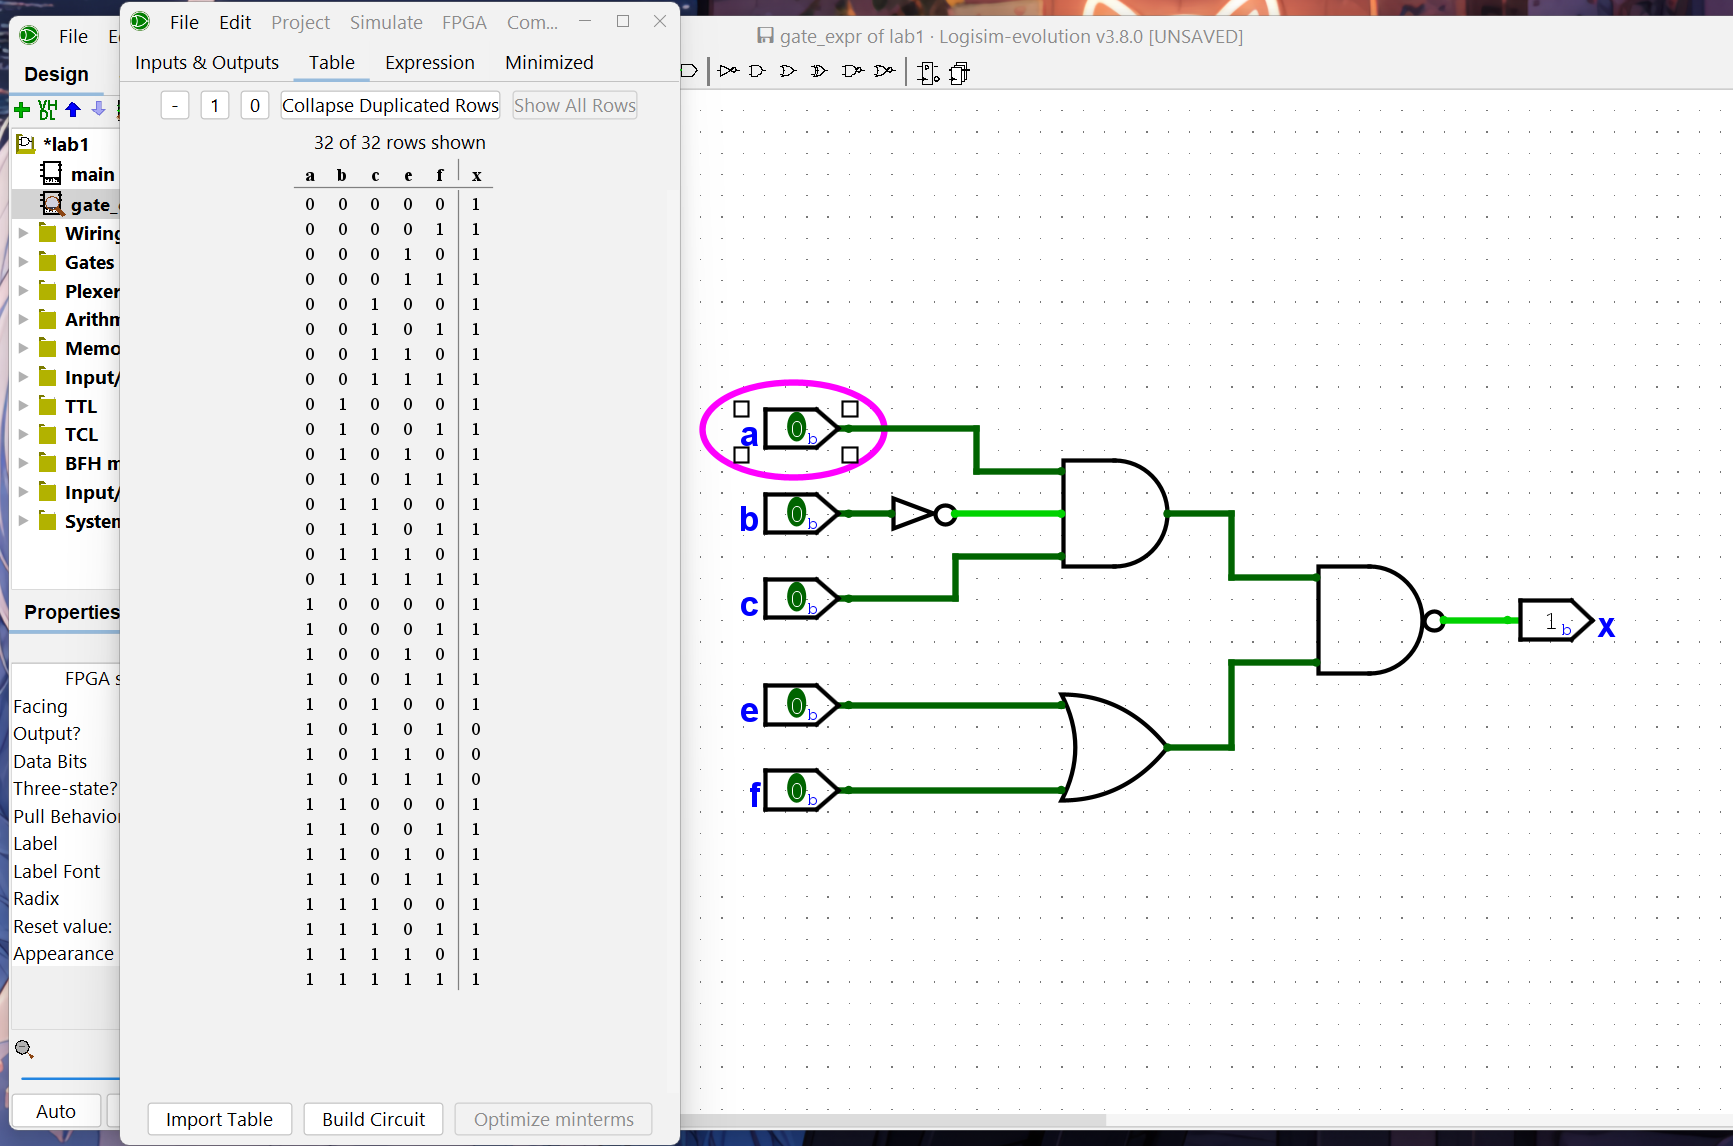
\includegraphics[width=0.98\textwidth]{0_gate_expr.png}
\caption{多输入门电路及全部 32 行真值表}
\label{fig:gate}
\end{figure}

图\ref{fig:gate}右侧为实际门级连接，左侧组合分析窗口显示全部 32 行。表头依次为 $a,b,c,e,f,x$，与实际电路的引脚命名一致。图中当前五个输入均为零，虽然取反后的 $b$ 为一，但与门中 $a,c$ 为零，最后与非门输出为一。

完整表中只有 $10101,10110,10111$ 三组输入使输出为零，顺序按 $a,b,c,e,f$ 解释。这与式\eqref{eq:gate}要求的 $a=1,b=0,c=1,e+f=1$ 完全一致。其余 29 组输出为一，说明非门、三输入与门、或门和最终与非门的连接关系符合目标表达式。

\subsection{二选一复用器验证}

\begin{figure}[H]
\centering
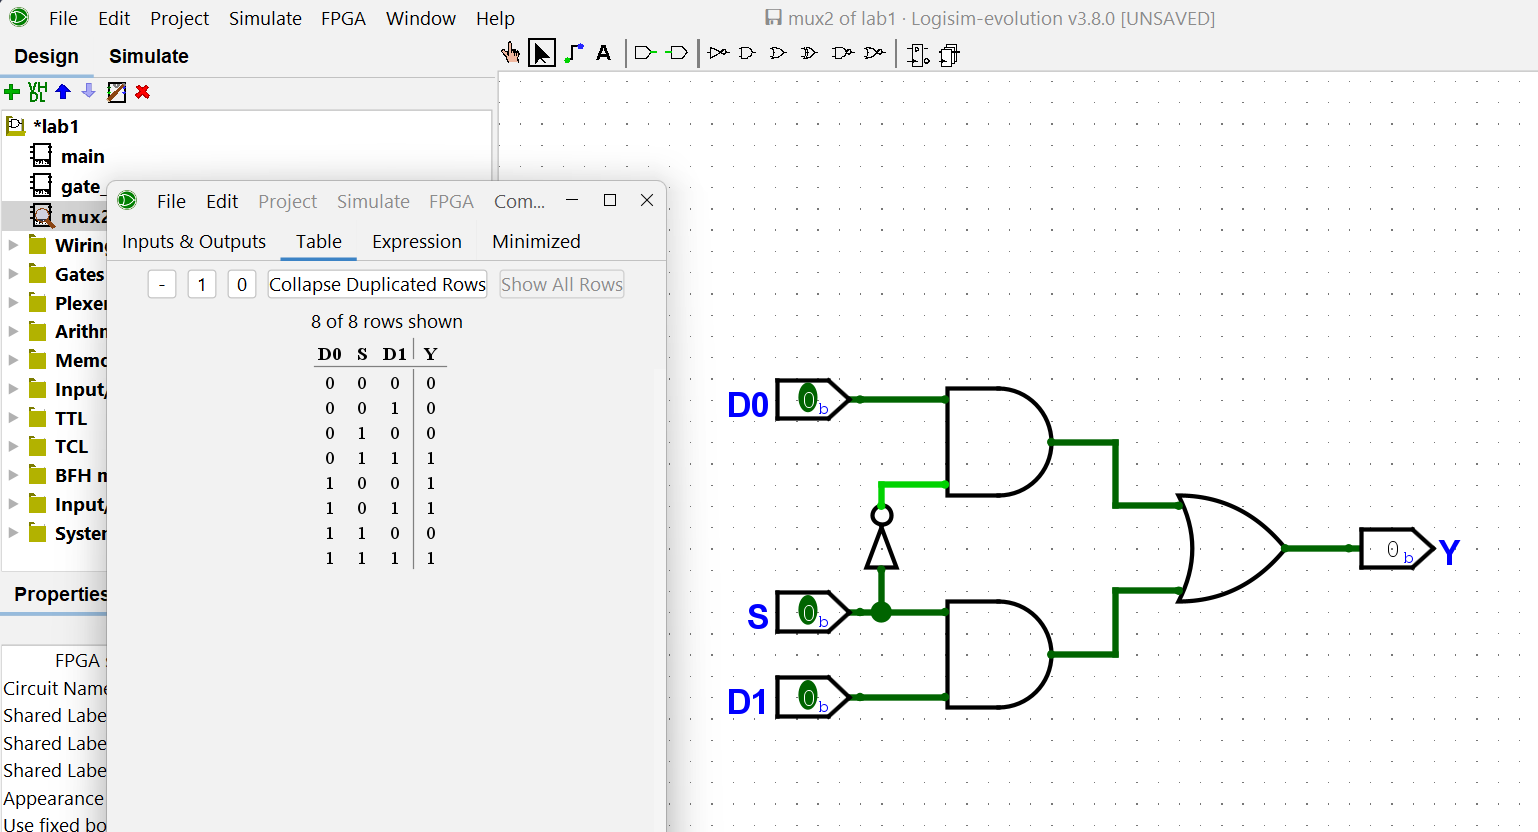
\includegraphics[width=0.98\textwidth]{1_mux2.png}
\caption{二选一复用器门级实现及八行真值表}
\label{fig:mux2}
\end{figure}

图\ref{fig:mux2}中，上支路将 $D_0$ 与 $\overline S$ 相与，下支路将 $D_1$ 与 $S$ 相与，再由或门输出。左侧表头的顺序是 $D_0,S,D_1,Y$，不能直接套用其他排列顺序读取。

在 $S=0$ 的各行，$Y$ 始终等于 $D_0$，改变 $D_1$ 不影响结果；在 $S=1$ 的各行，$Y$ 始终等于 $D_1$，改变 $D_0$ 不影响结果。全部八行与选择关系一致，验证了两条支路互斥导通的逻辑功能。

\subsection{四选一复用器与层次化设计验证}

\begin{figure}[H]
\centering
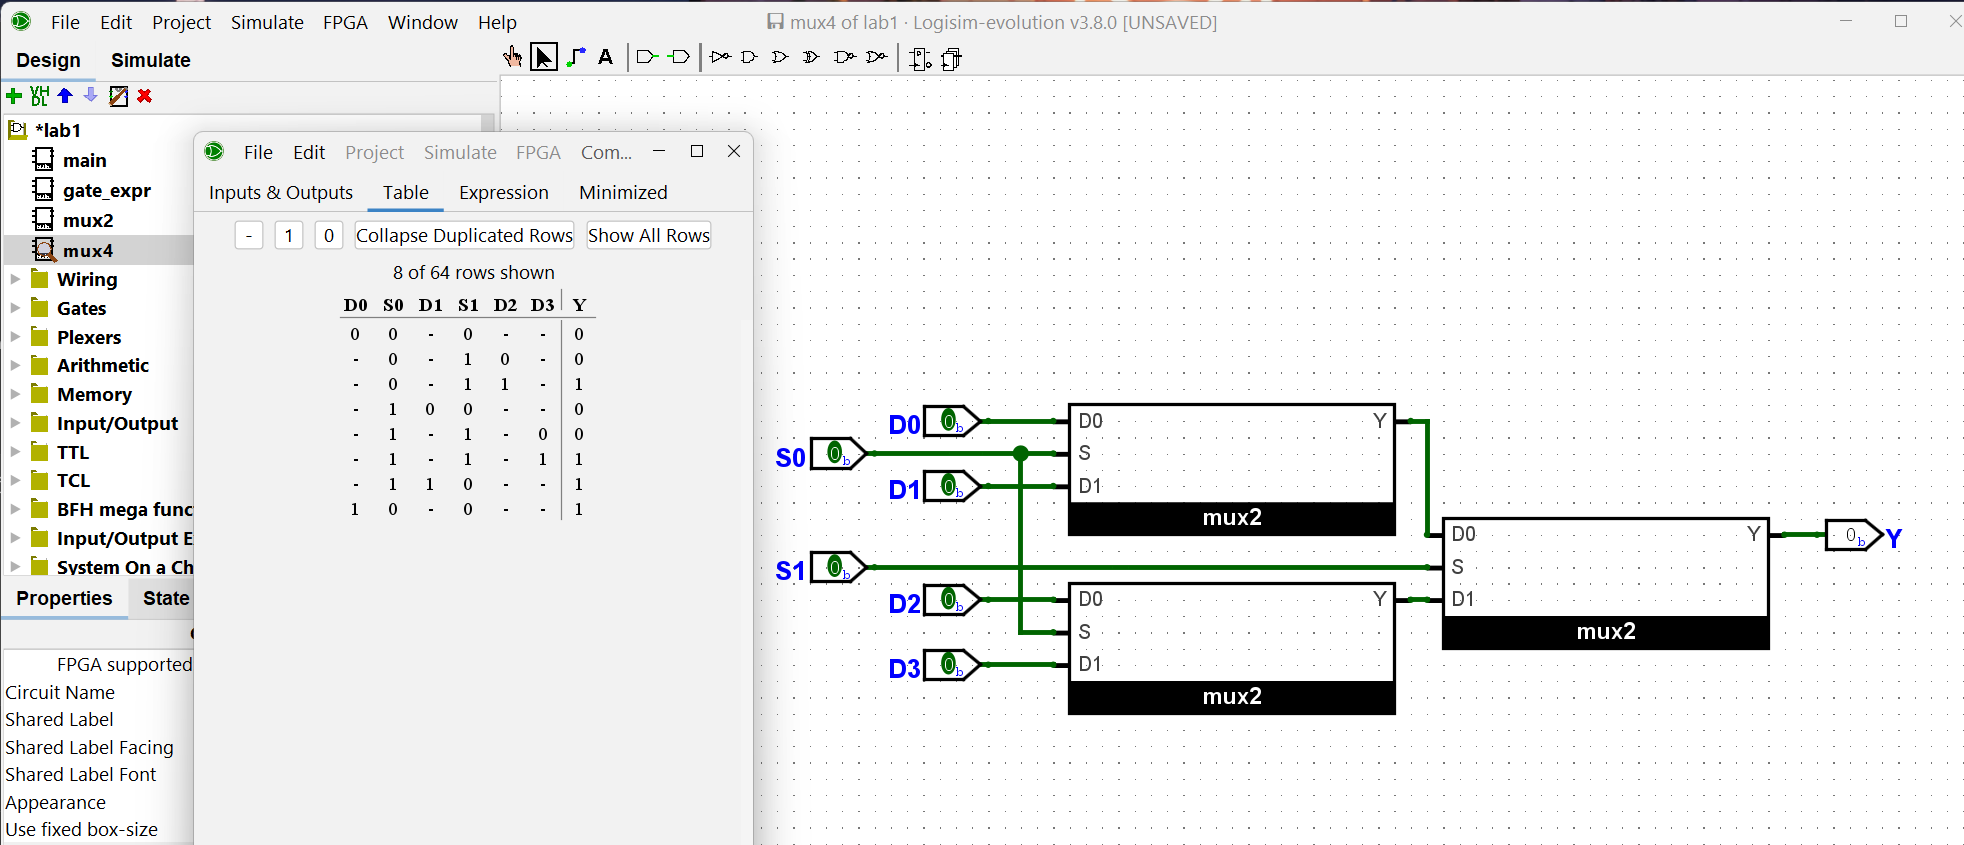
\includegraphics[width=0.98\textwidth]{2_mux4.png}
\caption{三个二选一子电路组成的四选一复用器及折叠真值表}
\label{fig:mux4}
\end{figure}

图\ref{fig:mux4}显示第一级两个实例共用 $S_0$，第二级实例由 $S_1$ 控制。上组输出接到第二级的 $D_0$，下组输出接到第二级的 $D_1$，因此没有交换两组的编号。

左侧窗口显示“8 of 64 rows shown”，表示 64 组输入被合并成八条规则。每个选择码对应选中数据为零或为一两种情况，其余三位数据均标为横线。表中例如 $S_1=1,S_0=0$ 时，$D_2=0$ 输出零，$D_2=1$ 输出一，其他数据不影响结果。这与表\ref{tab:mux4}一致，也说明三个二选一实例的层次连接正确。

\subsection{二线四线译码器仿真结果}

\begin{figure}[H]
\centering
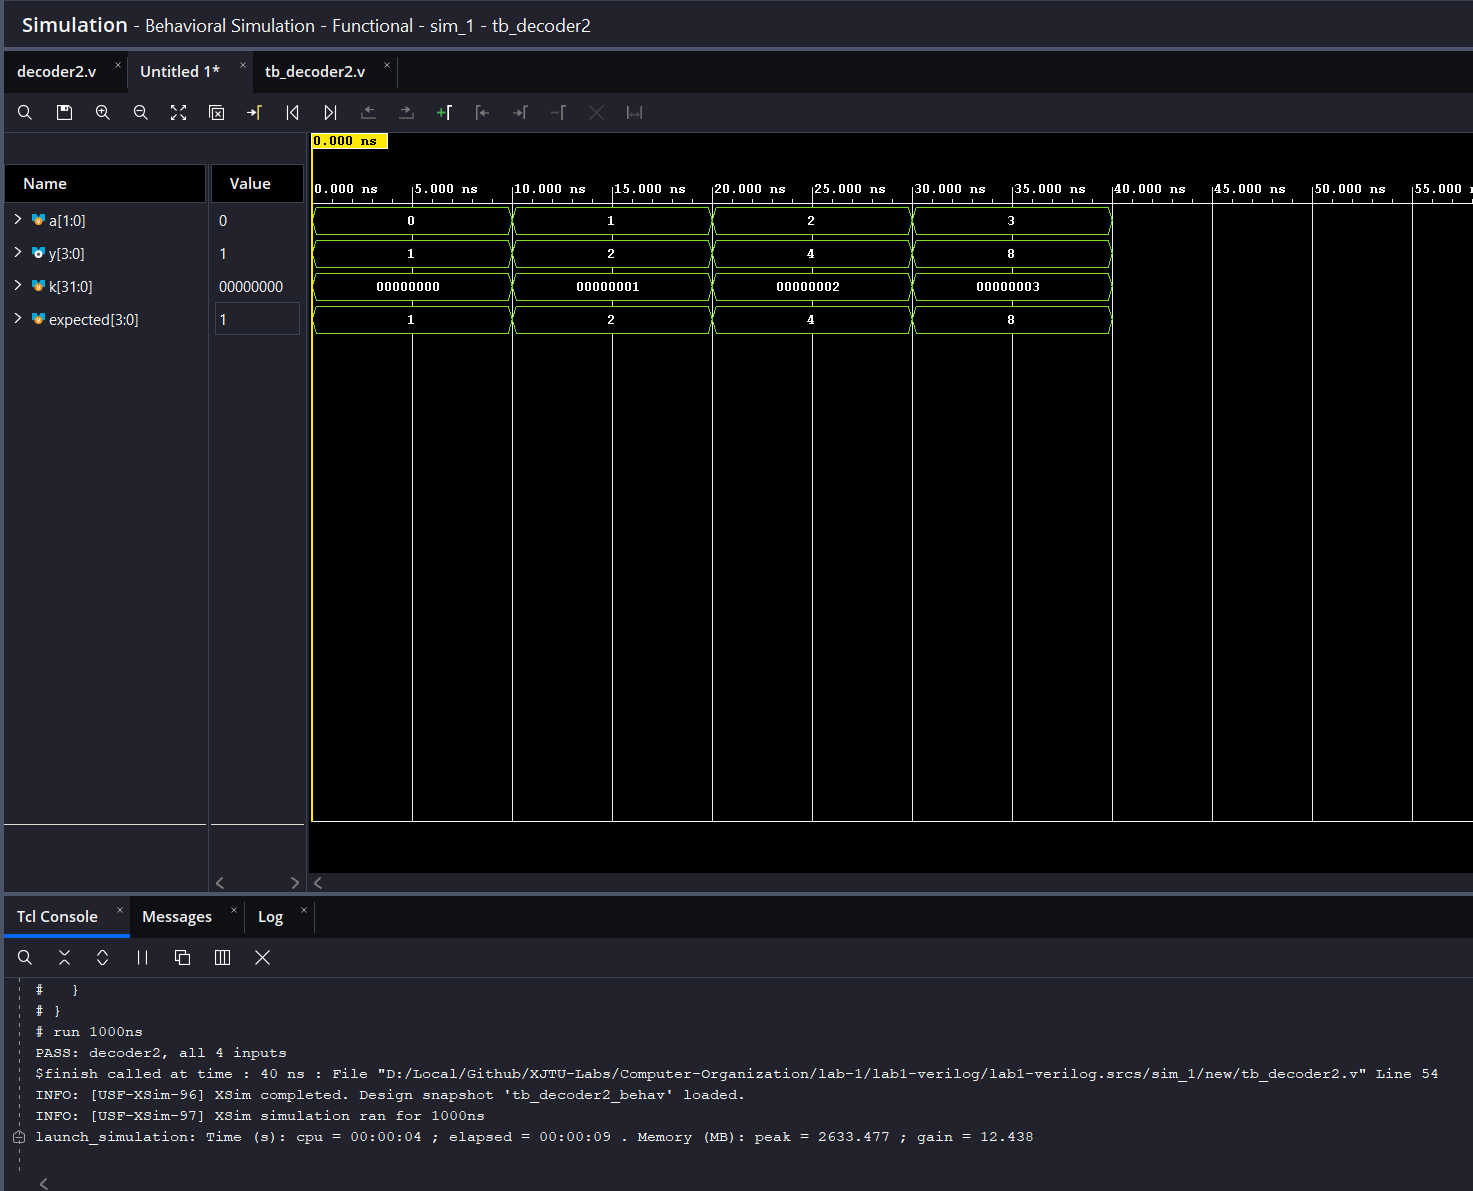
\includegraphics[width=0.94\textwidth]{3_decoder2_sim.png}
\caption{二线四线译码器的输入、输出、期望值及控制台结果}
\label{fig:decoder2}
\end{figure}

图\ref{fig:decoder2}中，输入每隔 10 ns 依次取 $0,1,2,3$，输出依次为 $1,2,4,8$，与 \texttt{expected} 波形逐段相同。其二进制形式分别为 $0001,0010,0100,1000$，每次只有对应输入编号的输出位为一。

控制台中的关键结果为：
\begin{lstlisting}[language={},numbers=none,caption={二线四线译码器的通过提示与结束时刻}]
PASS: decoder2, all 4 inputs
$finish called at time : 40 ns
\end{lstlisting}

第一行说明程序执行完全部四次比较，没有进入失败分支；第二行给出 $4\times10=40$ ns 的正常结束时刻。截图中还出现工具执行的 \texttt{run 1000ns}，但测试平台可以通过 \texttt{\$finish} 提前结束，所以不能把该运行命令的时间上限解释为电路必须仿真满 1000 ns。

\subsection{三线八线译码器仿真结果}

\begin{figure}[H]
\centering
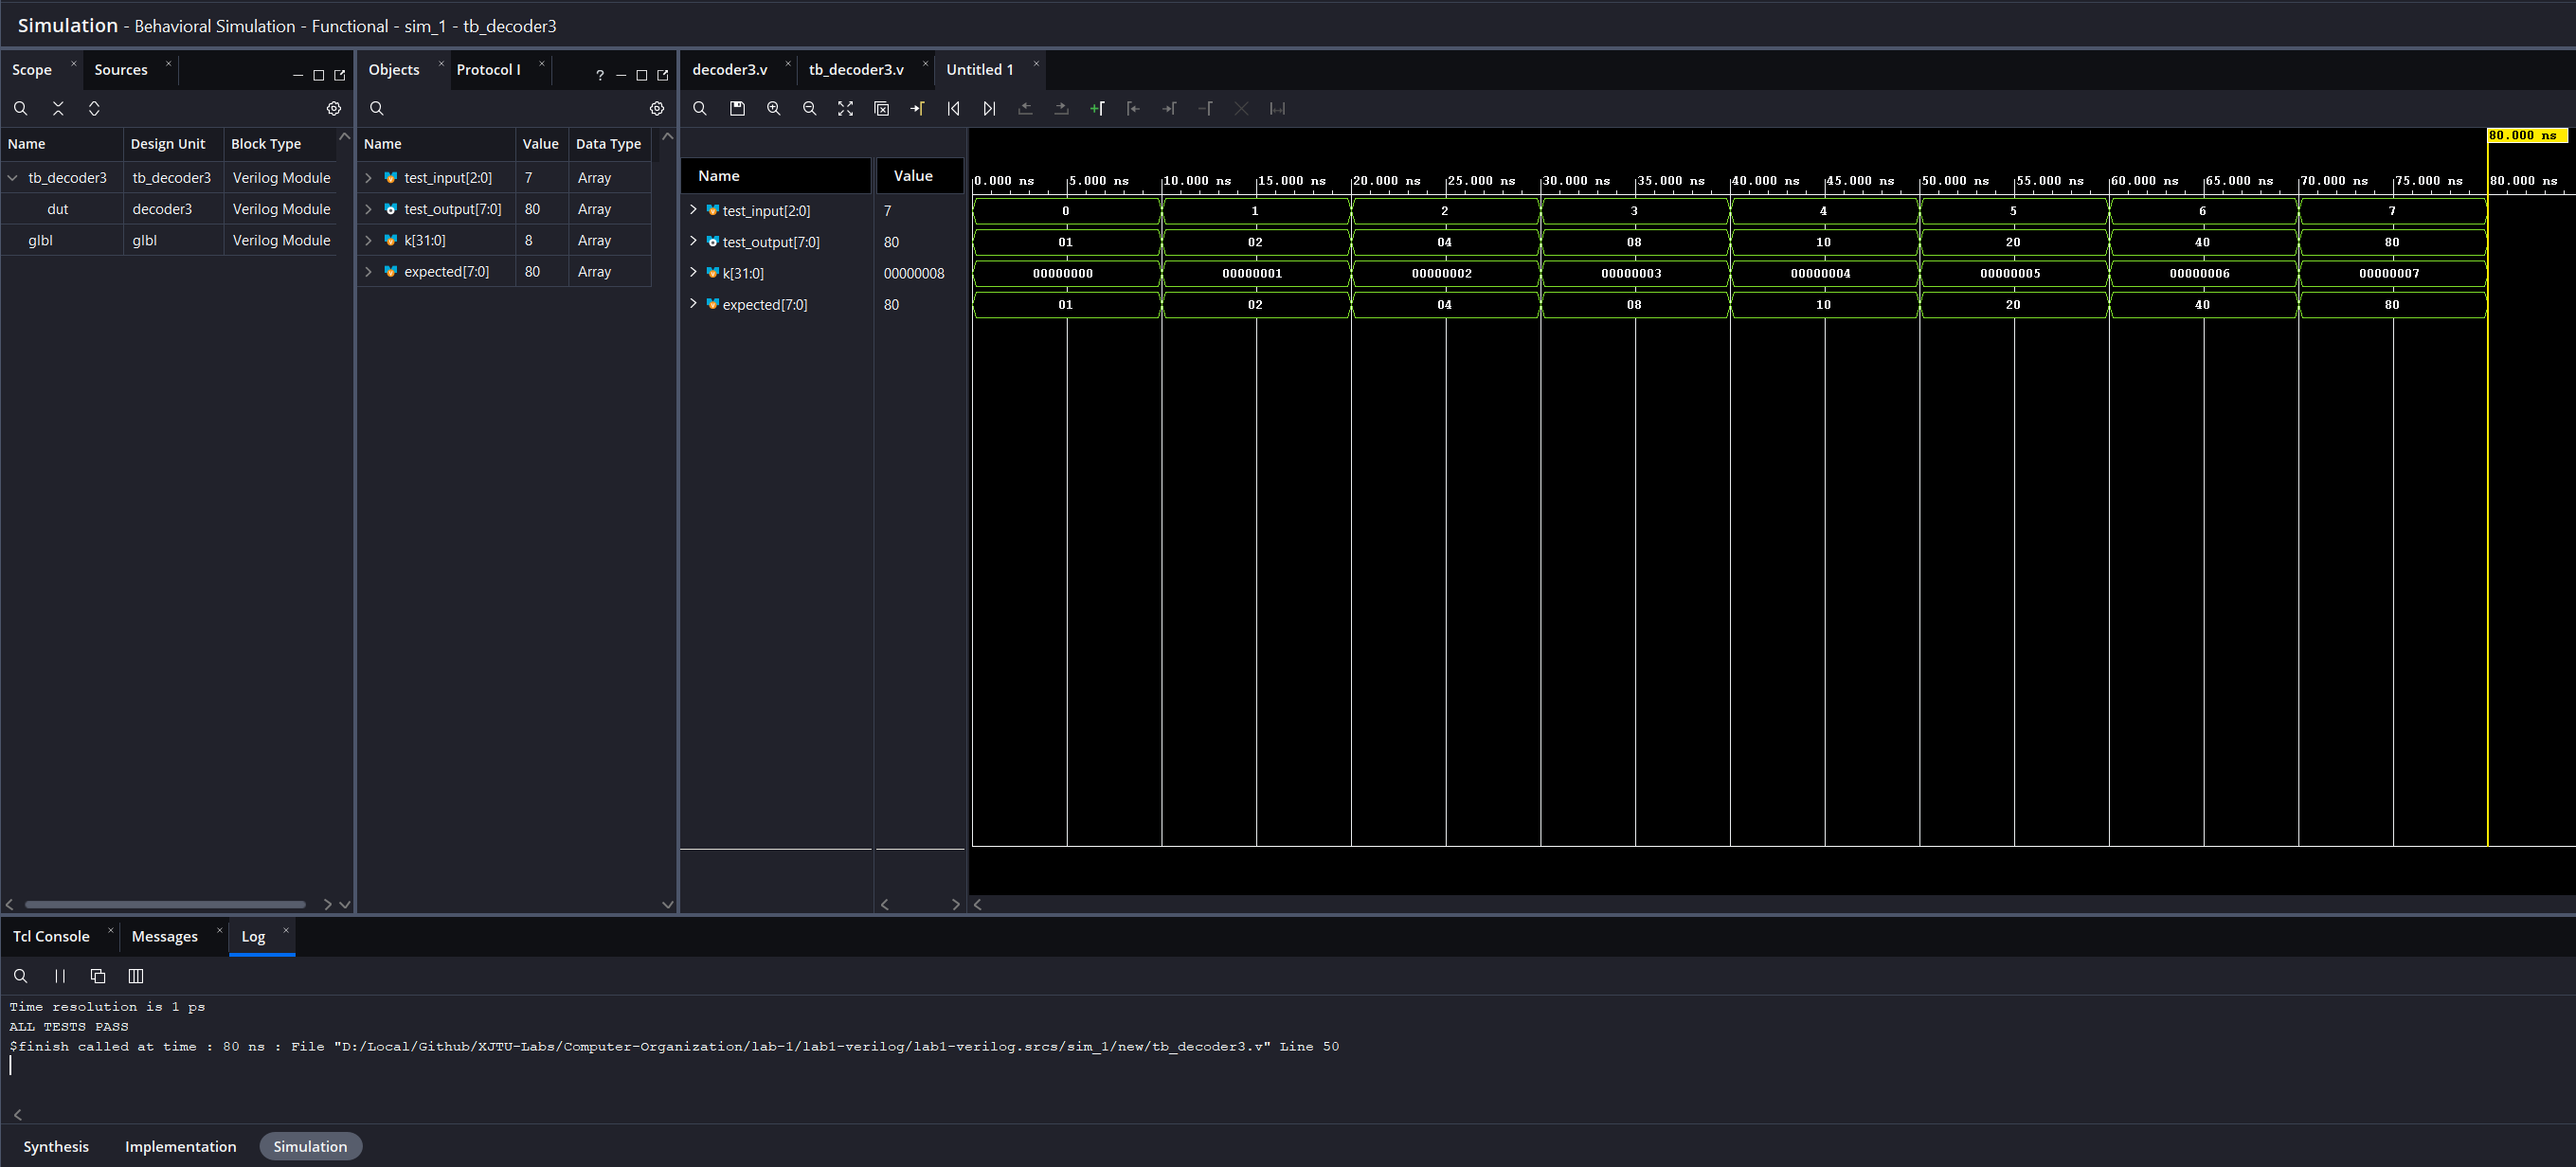
\includegraphics[width=\textwidth]{4_decoder3_sim.png}
\caption{三线八线译码器在 80 ns 内完成全部输入测试}
\label{fig:decoder3}
\end{figure}

图\ref{fig:decoder3}中输入从零递增到七，输出显示为十六进制序列 \texttt{01,02,04,08,10,20,40,80}，并始终与期望值相同。这里的 \texttt{10} 表示十六进制 $10$，即二进制 $00010000$；\texttt{80} 表示二进制 $10000000$，不是十进制八十。按正确进制读取后，可以看出有效位逐次从最低位移动到最高位。

\begin{table}[H]
\centering
\caption{三线八线译码器波形的逐段解释}
\label{tab:decoder3-wave}
\begin{tabular}{cccc}
\toprule
时间区间 / ns & 输入 $a$ & 输出十六进制 & 输出二进制 \\
\midrule
$[0,10)$ & 000 & 01 & 00000001 \\
$[10,20)$ & 001 & 02 & 00000010 \\
$[20,30)$ & 010 & 04 & 00000100 \\
$[30,40)$ & 011 & 08 & 00001000 \\
$[40,50)$ & 100 & 10 & 00010000 \\
$[50,60)$ & 101 & 20 & 00100000 \\
$[60,70)$ & 110 & 40 & 01000000 \\
$[70,80)$ & 111 & 80 & 10000000 \\
\bottomrule
\end{tabular}
\end{table}

表\ref{tab:decoder3-wave}将图中的数值转换成统一的二进制解释。所有输出既满足单热性，又满足有效位编号等于输入数值的要求。截图在 80 ns 处结束，循环变量最终为八，表示零至七的八组激励已经完成。

\begin{lstlisting}[language={},numbers=none,caption={三线八线译码器的通过提示与结束时刻}]
ALL TESTS PASS
$finish called at time : 80 ns
\end{lstlisting}

上述文本与截图底部日志一致。通过提示位于外层循环之后，说明八次比较全部完成；80 ns 则与测试平台设置的八组 10 ns 间隔一致。

\subsection{Logisim 优先编码器的真值表验证}

\begin{figure}[H]
\centering
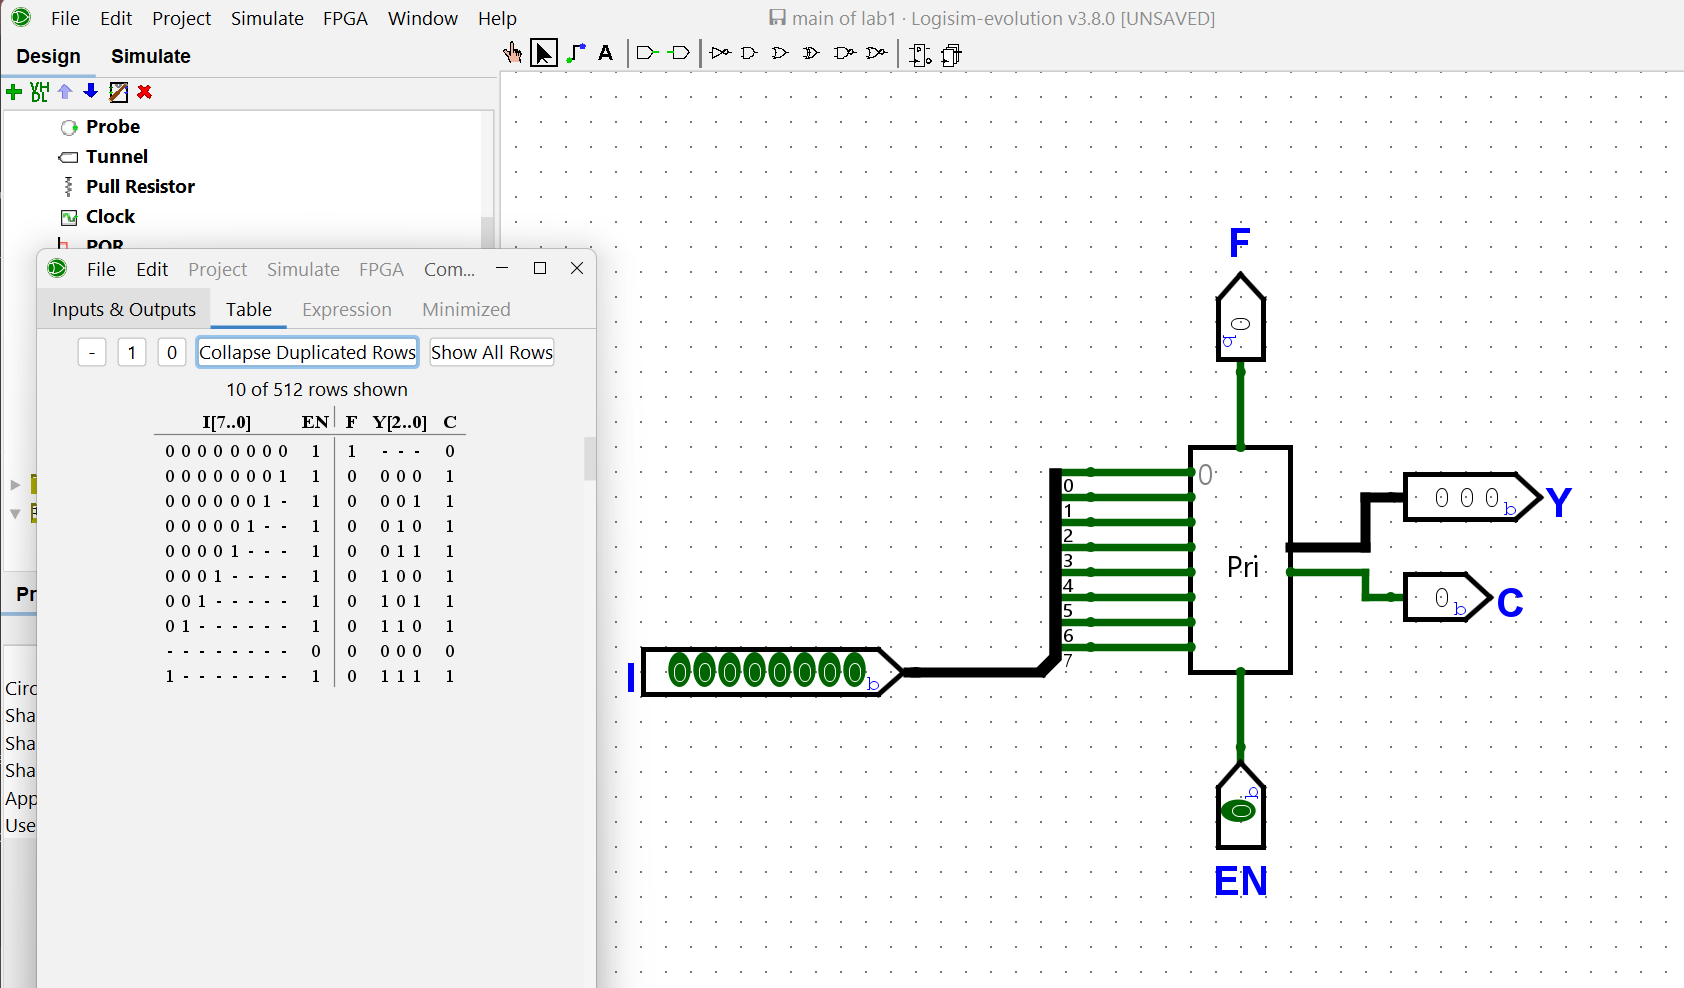
\includegraphics[width=0.98\textwidth]{5_priority8_logisim_test.png}
\caption{Logisim 优先编码器的接口连接与十条折叠规则}
\label{fig:priority-logisim}
\end{figure}

图\ref{fig:priority-logisim}中，八位输入总线经分线器连接到编号为零至七的输入，底部为使能 $EN$，上部和右下部分别为 $F$ 和 $C$。截图当前使能为零，因此输出为 $F=0,C=0,Y=000$。

组合分析窗口显示“10 of 512 rows shown”。九位输入包括八位数据和一位使能，共有 $2^9=512$ 种确定输入。十条折叠规则分别涵盖禁用状态、使能且无有效输入，以及八种最高有效位编号。横线表示在该条件下无关的位，例如输入最高位为一时，其余七位无论取何值，编码结果均为 $111$。使能且数据全零的行将 $Y$ 标为无关项，因此不能用该行证明零输入有有效的三位编号。

\subsection{Verilog 优先编码器仿真结果}

\begin{figure}[H]
\centering
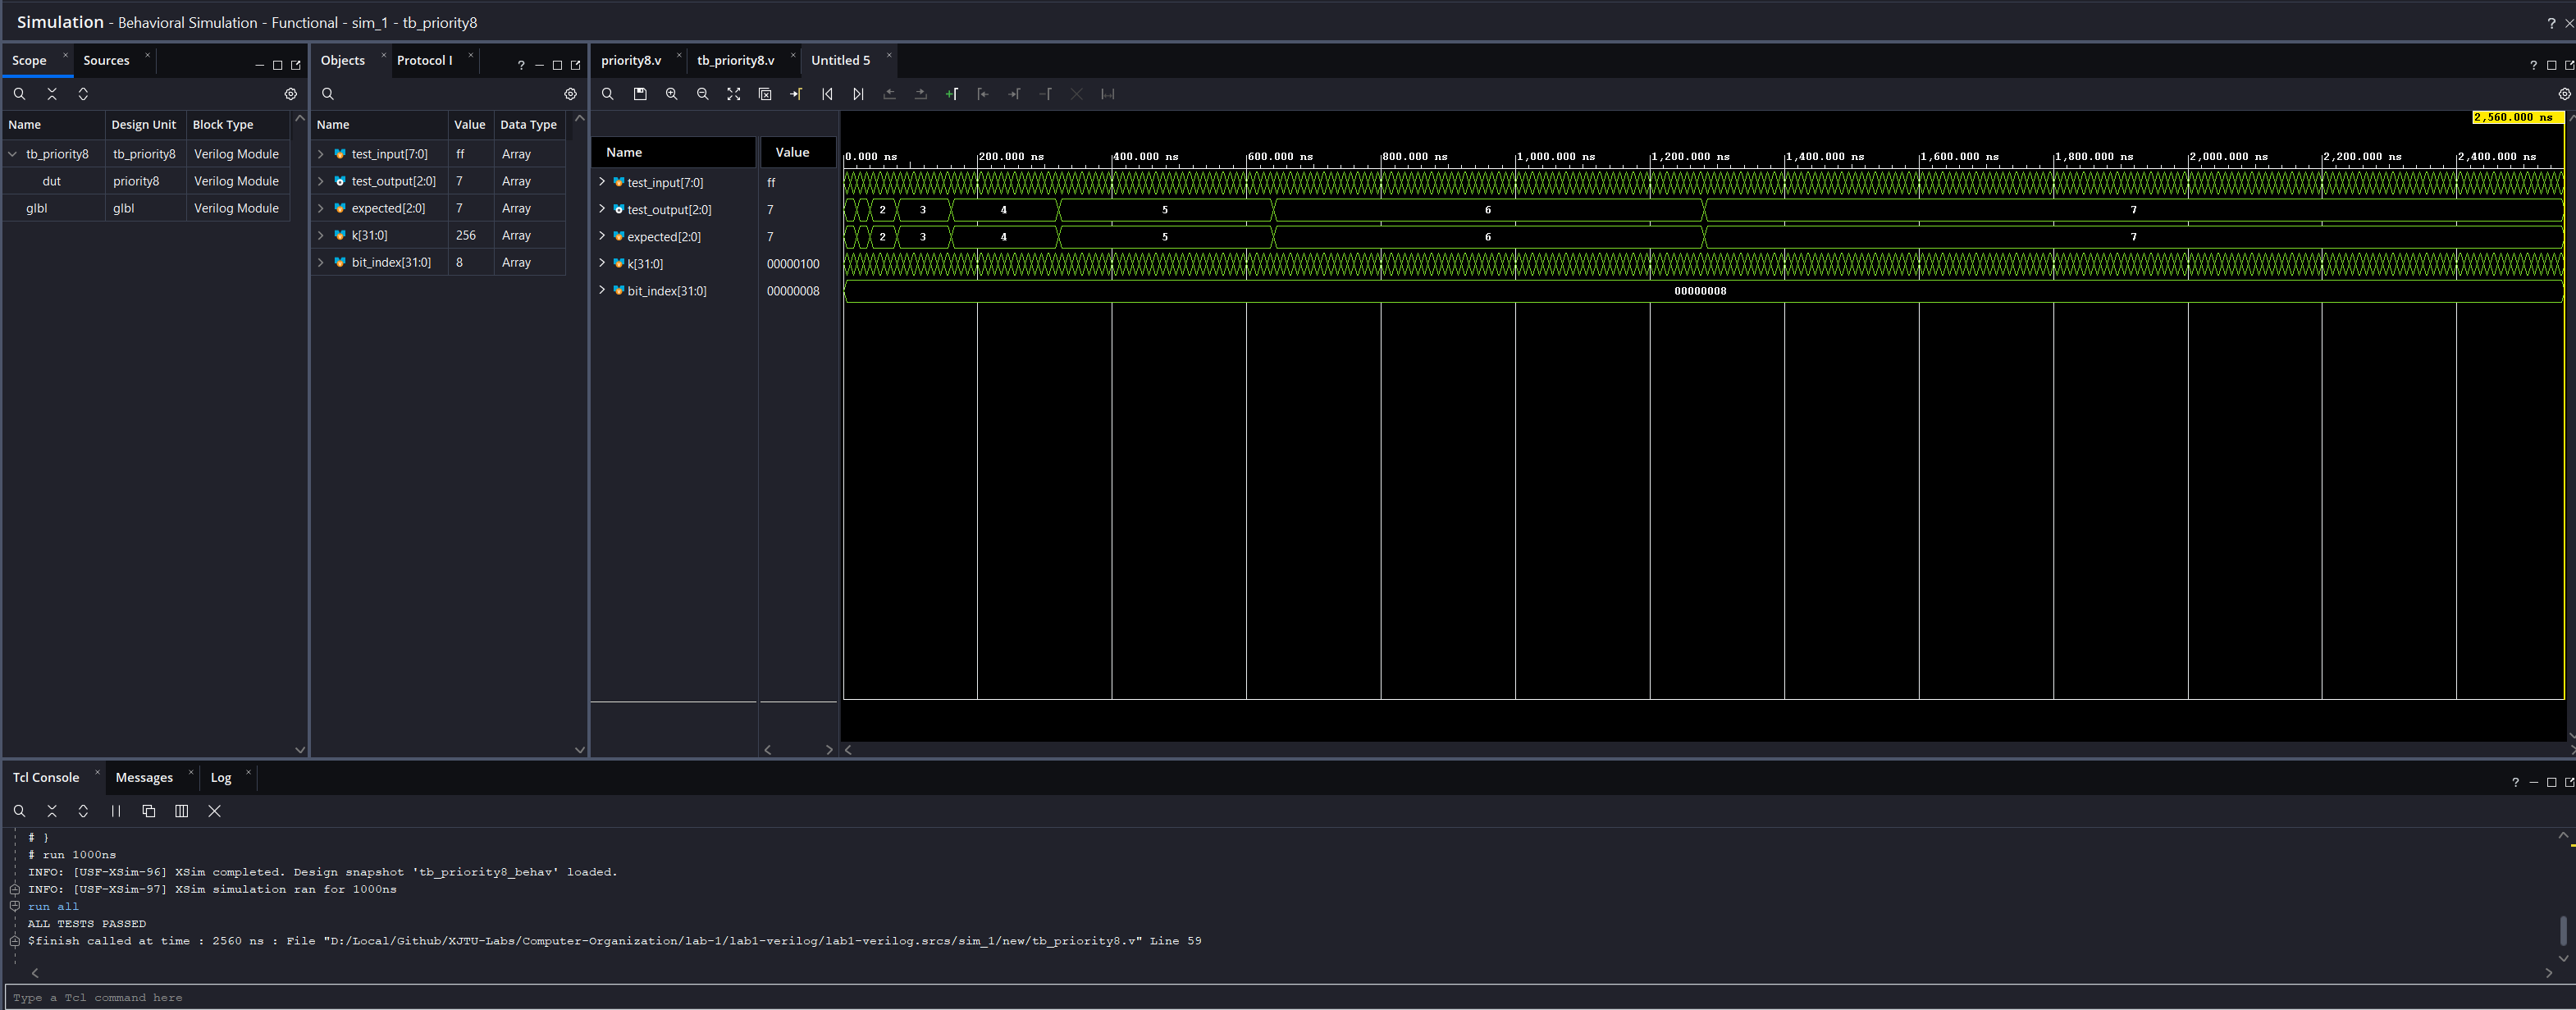
\includegraphics[width=\textwidth]{6_priority8_sim.png}
\caption{优先编码器完成 256 组穷举测试后的波形与结束输出}
\label{fig:priority-vivado}
\end{figure}

图\ref{fig:priority-vivado}中，八位 \texttt{test\_input} 从零递增到十六进制 \texttt{ff}，实际输出和期望输出均呈阶梯状。当输入最高有效位改变时，输出编号才发生变化；输入低位继续变化但最高有效位不变时，输出保持不变。这正是优先编码器的功能。

\begin{table}[H]
\centering
\caption{递增输入下优先编码器输出的分段规律}
\label{tab:priority-range}
\begin{tabular}{ccc}
\toprule
输入数值范围（十进制） & 时间区间 / ns & 输出编号 \\
\midrule
0、1 & $[0,20)$ & 0 \\
2--3 & $[20,40)$ & 1 \\
4--7 & $[40,80)$ & 2 \\
8--15 & $[80,160)$ & 3 \\
16--31 & $[160,320)$ & 4 \\
32--63 & $[320,640)$ & 5 \\
64--127 & $[640,1280)$ & 6 \\
128--255 & $[1280,2560)$ & 7 \\
\bottomrule
\end{tabular}
\end{table}

表\ref{tab:priority-range}解释了图中后半段输出长时间保持七的原因：从 128 开始，输入最高位始终为一，所有低位都不再影响结果。结束时输入为 \texttt{ff}，实际输出和期望值均为七；外层循环变量已增加到 256，内层变量为八，它们都是测试循环的结束状态，并非编码器输出。

截图和仿真日志中保留的关键文本如下：
\begin{lstlisting}[language={},numbers=none,caption={优先编码器从默认运行时长继续至正常结束}]
run 1000ns
run all
ALL TESTS PASSED
$finish called at time : 2560 ns
\end{lstlisting}

第一条命令只推进 1000 ns。在每组激励间隔 10 ns 的条件下，完整测试需要 $256\times10=2560$ ns，因此运行到 1000 ns 时尚未到达循环之后的成功提示。程序仅在不匹配时打印失败信息，若前面没有发现错误，暂停时没有调试输出属于预期现象。继续执行 \texttt{run all} 后，剩余测试完成，才输出成功提示并在 2560 ns 调用 \texttt{\$finish}。这说明最初现象来自运行时间设置，并非优先编码器发生了停滞。

\subsection{验证结论与适用范围}

三个 Verilog 测试平台均在独立目录重新编译并运行，分别在 40 ns、80 ns 和 2560 ns 输出与截图一致的成功提示，没有进入代码中的失败分支。结合 Logisim 真值表，可以确认本次保存的门电路、二级复用结构以及三个 Verilog 模块在已定义的二进制输入范围内满足设计功能。

测试平台的 10 ns 等待是激励之间的间隔，不代表电路传播延时为 10 ns。RTL 行为仿真也不能据此给出最高工作频率、板级毛刺或真实门延时结论。优先编码器的全零输入输出零属于本实现的接口约定；若系统需要判断有效性，应增加有效标志，而不能只检查三位编码结果。

\section{总结}

本实验通过 Logisim 和 Verilog 两种方式完成了组合逻辑的设计与验证。门电路部分将布尔表达式转换为实际连线，并用全部 32 行真值表检查；复用器部分由二选一模块构造四选一结构，验证了模块复用和分层设计的方法；编码与译码部分明确了最高位优先、单热输出和使能状态等概念。

Verilog 设计中，译码器使用连续赋值描述并行逻辑，优先编码器使用完整的组合过程块描述选择优先级。测试平台通过穷举输入、计算独立期望值和自动比较，提高了验证覆盖范围。三组测试分别完成 4、8 和 256 组输入检查，均正常结束。

实验中的两个细节值得保留：一是应根据测试总时长选择仿真运行范围，默认 1000 ns 不足以覆盖 2560 ns 的优先编码器测试；二是期望值应尽量按每组输入重新初始化，避免未来改变激励顺序时产生旧值残留。后续可以增加有效输出、零输入重复测试和未知态专项检查，并在需要时进一步完成 FPGA 硬件验证。

\clearpage
\section*{附录：实验源代码}
\addcontentsline{toc}{section}{附录：实验源代码}

以下直接嵌入本次工程中全部三个模块设计源代码与三个仿真源代码，包含原有时间尺度声明及自动生成的注释。代码均为现有文件的完整内容，没有用外部文件引用替代。附录之后给出仿真操作命令及其说明。

\subsection*{A.1 二线四线译码器设计}

\begin{lstlisting}[caption={decoder2.v 完整源码}]
`timescale 1ns / 1ps
//////////////////////////////////////////////////////////////////////////////////
// Company: 
// Engineer: 
// 
// Create Date: 10/21/2026 04:27:00 AM
// Design Name: 
// Module Name: decoder2
// Project Name: 
// Target Devices: 
// Tool Versions: 
// Description: 
// 
// Dependencies: 
// 
// Revision:
// Revision 0.01 - File Created
// Additional Comments:
// 
//////////////////////////////////////////////////////////////////////////////////


module decoder2(
    input wire [1:0] a,
    output wire [3:0] y
    );
   
    assign y[0] = ~a[0] & ~a[1];    
    assign y[1] =  a[0] & ~a[1];    
    assign y[2] = ~a[0] &  a[1];    
    assign y[3] =  a[0] &  a[1];   
     
endmodule
\end{lstlisting}

该模块的两个输入位共同选择四个输出之一。每条连续赋值只驱动一个输出位，分别表示输入为零、一、二、三的条件。源码先写低位再写高位，例如 \texttt{a[0] \& \~{}a[1]} 对应输入二进制 $01$；逻辑与满足交换律，书写顺序与正文公式不同但结果一致。模块没有时钟和过程状态，输入变化后各输出按表达式更新。文件开头的工程信息注释不参与电路功能。


\subsection*{A.2 二线四线译码器仿真}

\begin{lstlisting}[caption={tb\_decoder2.v 完整源码}]
`timescale 1ns / 1ps
//////////////////////////////////////////////////////////////////////////////////
// Company: 
// Engineer: 
// 
// Create Date: 10/21/2026 04:42:20 AM
// Design Name: 
// Module Name: tb_decoder2
// Project Name: 
// Target Devices: 
// Tool Versions: 
// Description: 
// 
// Dependencies: 
// 
// Revision:
// Revision 0.01 - File Created
// Additional Comments:
// 
//////////////////////////////////////////////////////////////////////////////////


`timescale 1ns/1ps

module tb_decoder2;

    reg  [1:0] a;
    wire [3:0] y;

    integer k;
    reg [3:0] expected;

    decoder2 dut (
        .a(a),
        .y(y)
    );

    initial begin
        a = 2'b00;

        for (k = 0; k < 4; k = k + 1) begin
            a = k;
            expected = 4'b0001 << k;
            #10;

            if (y !== expected) begin
                $display("FAIL: a=%b y=%b expected=%b",
                         a, y, expected);
                $fatal(1, "decoder2 failed");
            end
        end

        $display("PASS: decoder2, all 4 inputs");
        $finish;
    end

endmodule
\end{lstlisting}

测试平台把 \texttt{a} 声明为过程驱动信号，将待测输出接到 \texttt{y}，再通过实例 \texttt{dut} 完成端口连接。外层循环穷举四个输入，四位常量左移生成对应单热期望值，等待 10 ns 后用 \texttt{!==} 比较。失败时先打印输入、实际输出和期望值，再用 \texttt{\$fatal} 终止；全部通过后打印成功提示并调用 \texttt{\$finish}。源码有两条等价的时间尺度声明，它们不会把延时相加，也不会使总时长翻倍；本测试仍在 40 ns 完成。


\subsection*{A.3 三线八线译码器设计}

\begin{lstlisting}[caption={decoder3.v 完整源码}]
`timescale 1ns / 1ps
//////////////////////////////////////////////////////////////////////////////////
// Company: 
// Engineer: 
// 
// Create Date: 10/22/2026 04:15:25 PM
// Design Name: 
// Module Name: decoder3
// Project Name: 
// Target Devices: 
// Tool Versions: 
// Description: 
// 
// Dependencies: 
// 
// Revision:
// Revision 0.01 - File Created
// Additional Comments:
// 
//////////////////////////////////////////////////////////////////////////////////


module decoder3(
    input  wire [2:0] a,
    output wire [7:0] y
    );
    
    assign y[0] = ~a[2] & ~a[1] & ~a[0];
    assign y[1] = ~a[2] & ~a[1] &  a[0];
    assign y[2] = ~a[2] &  a[1] & ~a[0];
    assign y[3] = ~a[2] &  a[1] &  a[0];
    assign y[4] =  a[2] & ~a[1] & ~a[0];
    assign y[5] =  a[2] & ~a[1] &  a[0];
    assign y[6] =  a[2] &  a[1] & ~a[0];
    assign y[7] =  a[2] &  a[1] &  a[0];
    
endmodule
\end{lstlisting}

该模块用八条连续赋值列出全部三变量最小项。对任意确定的三位输入，八个条件中恰好一个成立，因此输出既是单热码，也能按有效位位置还原输入编号。例如输入 $101$ 时只有第五号输出条件成立，得到 \texttt{8'b00100000}。所有输出都持续被驱动，无须用默认分支保持旧值。


\subsection*{A.4 三线八线译码器仿真}

\begin{lstlisting}[caption={tb\_decoder3.v 完整源码}]
`timescale 1ns / 1ps
//////////////////////////////////////////////////////////////////////////////////
// Company: 
// Engineer: 
// 
// Create Date: 10/22/2026 04:19:36 PM
// Design Name: 
// Module Name: tb_decoder3
// Project Name: 
// Target Devices: 
// Tool Versions: 
// Description: 
// 
// Dependencies: 
// 
// Revision:
// Revision 0.01 - File Created
// Additional Comments:
// 
//////////////////////////////////////////////////////////////////////////////////


module tb_decoder3;

    reg  [2:0] test_input;
    wire [7:0] test_output;
    
    integer k;
    reg [7:0]  expected;
    
    decoder3 dut (
        .a(test_input),
        .y(test_output)
    );
    
    initial begin
    
        for (k = 0; k < 8; k = k + 1) begin
            test_input = k;
            expected = 8'b00000001 << k;
            #10;
            
            if (test_output !== expected) begin
                $display("FAIL: test_input = %b, test_output = %b, expected = %b", test_input, test_output, expected);
                $fatal(1, "decoder3 failed");
            end            
        end
    
        $display("ALL TESTS PASS");
        $finish;
    
    end 

endmodule
\end{lstlisting}

该测试从 \texttt{k=0} 开始立即给 \texttt{test\_input} 赋值，因此虽然没有单独的初始赋值语句，也能在第一组测试开始时得到确定输入。每轮利用八位单热常量左移产生期望值，10 ns 后比较实际输出。八次比较累计 80 ns，全部匹配才打印 \texttt{ALL TESTS PASS}。相比二线四线测试，这里扩展了信号位宽和循环范围，验证方法保持一致。


\subsection*{A.5 八线三线优先编码器设计}

\begin{lstlisting}[caption={priority8.v 完整源码}]
`timescale 1ns / 1ps
//////////////////////////////////////////////////////////////////////////////////
// Company: 
// Engineer: 
// 
// Create Date: 10/22/2026 05:02:04 PM
// Design Name: 
// Module Name: priority8
// Project Name: 
// Target Devices: 
// Tool Versions: 
// Description: 
// 
// Dependencies: 
// 
// Revision:
// Revision 0.01 - File Created
// Additional Comments:
// 
//////////////////////////////////////////////////////////////////////////////////


module priority8(
    input  wire  [7:0] i,
    output reg   [2:0] y
    );
    
    always @* begin
    
        if      (i[7]) y = 3'd7;
        else if (i[6]) y = 3'd6;
        else if (i[5]) y = 3'd5;
        else if (i[4]) y = 3'd4;
        else if (i[3]) y = 3'd3;
        else if (i[2]) y = 3'd2;
        else if (i[1]) y = 3'd1;
        else           y = 3'd0;
        
    end
    
endmodule
\end{lstlisting}

组合过程块按第七位到第一位顺序判断，先满足的高位分支决定结果，其余低位不再影响输出。最后的默认分支将剩余情况统一输出为零，因此最低位有效和完全没有有效输入得到相同编码。输出使用三位宽度，足以容纳零至七；\texttt{always @*} 与完整赋值分支共同描述不依赖历史状态的组合逻辑。该源码没有使能和有效标志，不能把 Logisim 组件的额外状态端口理解为此模块已有的功能。


\subsection*{A.6 八线三线优先编码器仿真}

\begin{lstlisting}[caption={tb\_priority8.v 完整源码}]
`timescale 1ns / 1ps
//////////////////////////////////////////////////////////////////////////////////
// Company: 
// Engineer: 
// 
// Create Date: 10/23/2026 01:19:20 AM
// Design Name: 
// Module Name: tb_priority8
// Project Name: 
// Target Devices: 
// Tool Versions: 
// Description: 
// 
// Dependencies: 
// 
// Revision:
// Revision 0.01 - File Created
// Additional Comments:
// 
//////////////////////////////////////////////////////////////////////////////////


module tb_priority8;

    reg  [7:0] test_input;
    wire [2:0] test_output;
    reg  [2:0] expected;
    
    priority8 dut (
        .i(test_input),
        .y(test_output)
    );
    
    integer k;
    integer bit_index;
    
    initial begin
    
        expected = 3'b000;
    
        for (k = 0; k < 256; k = k + 1) begin
        
            test_input = k;
            
            // scan upward: the last asserted bit is the highest
            for (bit_index = 0; bit_index < 8; bit_index = bit_index + 1) begin
                if (test_input[bit_index]) expected = bit_index;
            end
            
            #10;
            
            if (test_output !== expected) begin
                $display("FAIL: test_input = %b, test_output = %b, expected = %b", test_input, test_output, expected);
                $fatal(1, "priority8 failed");
            end      
        end
        
        $display("ALL TESTS PASSED");
        $finish;
    
    end

endmodule
\end{lstlisting}

外层循环产生零至 255 的全部八位输入。内层循环按位号递增扫描，每发现一个置位输入就覆盖 \texttt{expected}，因此扫描结束时保留最高有效位编号。每组等待 10 ns 后比较，256 组累计 2560 ns。\texttt{expected} 只在循环之前清零，但当前递增顺序保证全零输入先被检查，后续非零输入都重新覆盖期望值，因而现有运行能够通过。为支持更一般的激励顺序，应将清零放到每轮外层循环内；本附录保持现有程序原样。成功提示位于所有测试之后，只有将仿真继续运行至循环完成，控制台才会显示 \texttt{ALL TESTS PASSED}。


\subsection*{A.7 仿真操作命令}

在 Vivado 已经打开相应测试平台的仿真会话后，可以直接使用以下 Tcl 命令继续运行：
\begin{lstlisting}[language={},numbers=none,caption={继续执行剩余仿真事件}]
run all
\end{lstlisting}

这条命令从当前仿真时刻继续执行，直到测试平台调用结束语句，或仿真遇到其他停止条件。对于当前优先编码器测试，从默认的 1000 ns 暂停点继续运行即可，不需要为增加运行时长修改硬件设计。

如果只需要从头观察已经编译的同一组测试，可以执行：
\begin{lstlisting}[language={},numbers=none,caption={重置时间并重新运行当前仿真}]
restart
run all
\end{lstlisting}

\texttt{restart} 将当前快照的仿真状态恢复到起点，随后 \texttt{run all} 重跑测试。若已经修改源代码，应保存并重新启动或重新编译仿真，不能仅依赖重置旧快照。切换电路时，还应把对应测试平台设为仿真顶层：译码器分别选择 \texttt{tb\_decoder2}、\texttt{tb\_decoder3}，优先编码器选择 \texttt{tb\_priority8}。


\end{document}
